\chapter{Scaling law: 법칙이 아니라 측정 가능한 가설부터}
\label{STC-S12}

Pre-training scaling은 통제된 data, parameter, compute와 loss의 관계를 다룬다. STC에는 previous
state, wake evidence, admission policy, memory medium, cycle count, future query reuse, validation과
publication이 추가되어 path-dependent하다. 따라서 ``accuracy versus sleep FLOPs'' 한 곡선은 state가
증가했는지, data가 좋아졌는지, future reuse가 달랐는지 구분하지 못한다.

동결 corpus의 어느 source도 보편적인 sleep-time scaling law를 확립하지 않는다.\claim{STC-C041}
\autocite{srcstc0034,srcstc0035,srcstc0050} 아래 식은 \measured{} accounting identity,
\analytical{} break-even, \fitcandidate{}, \hypothesis{}의 네 등급으로 분리한다. 관측 전 가설을
``law''라고 부르지 않는 것이 이 장의 가장 중요한 결과다.

\begin{figure}[htbp]
  \centering
  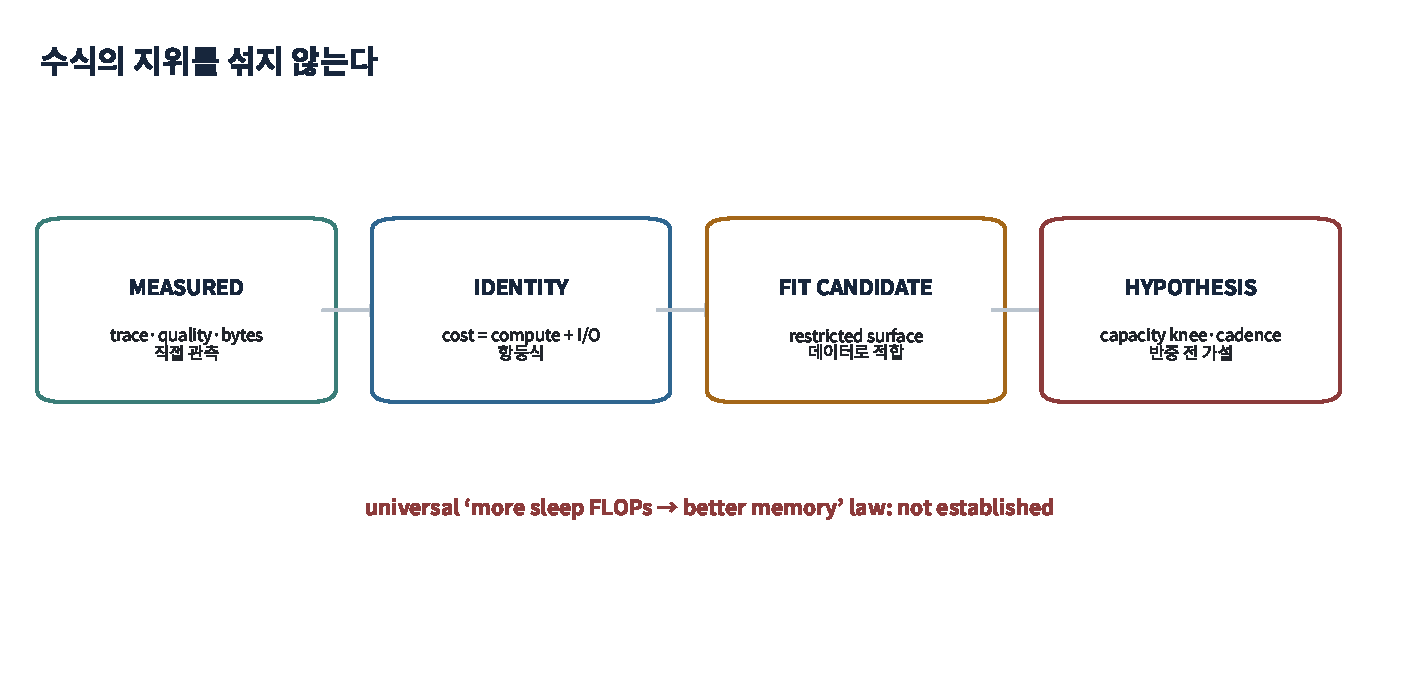
\includegraphics[width=0.98\textwidth]{figures/stc-f007.pdf}
  \caption{Scaling statement의 네 등급. Identity는 장부를 닫고, break-even은 제한된 가정 아래
  경계를 계산하며, fit candidate는 sweep에 맞추고, hypothesis는 반증 실험을 기다린다.}
  \stcfigure{STC-F007}
  \figsource{Original synthesis; SRC-STC-0035, SRC-STC-0050}{측정식에서 보편 법칙으로 갈수록 필요한 가정과 검증 범위가 증가하는 네 단계 사다리.}
  \label{fig:scaling-evidence-ladder}
\end{figure}

\section{State와 lifecycle work를 먼저 닫는 identity}

Answer-bearing retained state를 destination 하나로 축소하면 안 된다.

\begin{equation}
B_{retained}=B_r+B_e+B_l+B_p+B_a+B_v,
\label{eq:retained-state}
\end{equation}

여기서 $B_r$은 canonical/raw evidence, $B_e$는 text/vector/graph/index, $B_l$은 latent·KV·recurrent
state, $B_p$는 adapter/expert/weight delta, $B_a$는 optimizer·importance·router·teacher support,
$B_v$는 lineage·predecessor·rollback state다. Active summary bytes만 보고 ``압축률''을 계산하면 archive와
recovery copy가 사라진 것처럼 보이는 오류가 생긴다.

동시에 존재하는 candidate, pinned predecessor, migration, workspace, replica까지 더한 peak는

\begin{align}
B_{peak,state}(t)={}&B_{retained}(t)+B_{candidate}(t)+B_{pinned}(t)\nonumber\\
&+B_{migration}(t)+B_{workspace}(t)+B_{replica}(t),\\
B_{peak,physical}(t)={}&B_{base,resident}(t)+B_{peak,state}(t)+B_{execution}(t).
\end{align}

Physical maximum은 각 항의 서로 다른 시간대 high-water mark를 더하지 않고 같은 timestamp에서
평가한다. Separate wake/sleep fleet가 contention을 줄이면서 base model replica를 늘릴 수 있으므로
incremental state와 physical placement를 둘 다 보고해야 한다.

Full-history replay는 특히 위험하다. Cycle $t$에서 이전 task의 $m_i$개를 모두 replay하면

\begin{equation}
W_T=\sum_{t=1}^{T}\sum_{i=1}^{t}m_i
=\sum_{i=1}^{T}m_i(T-i+1).
\end{equation}

$m_i=m>0$이면 $W_T=mT(T+1)/2=\Theta(T^2)$다. Admission fraction을 일정 비율 줄이는 것만으로는
계수만 줄고 차수가 바뀌지 않는다. Bounded memory를 주장하려면 expire, compaction, coreset,
generated replay 또는 selective revisit가 실제로 lifetime work와 retained state를 제한하는지 보여야 한다.

\section{Valid reuse가 만드는 compile break-even}

Sleep artifact $i$의 가치에서 raw memory count나 sleep FLOPs보다 유용한 후보 변수는 valid reusable
evidence per lifecycle cost다.\claim{STC-C043}\autocite{srcstc0035,srcstc0043,srcstc0051}
그 이유는 compile이 한 번 비싸도 미래에 반복 사용되면 이득이고, 수천 개 memory를 만들었어도 다시
쓰이지 않으면 이득이 0이기 때문이다.

Stationary하고 quality가 같다는 제한된 가정에서 reuse break-even은

\begin{equation}
n^*=\frac{C_{compile}+C_{maint}}{\Delta C_{use}}.
\label{eq:reuse-break-even}
\end{equation}

Validity survival과 discount를 넣으면 horizon $H$의 expected valid reuse는

\begin{equation}
R_i(H)=\int_0^H \lambda_i(t)S_i(t)e^{-\omega t}\,dt.
\end{equation}

Promotion은 $R_i(H)\Delta U_{ij}$가 compile, serve, governance, risk cost의 합보다 클 때만 후보가 된다.
Future reuse를 oracle로 쓰지 않기 위해 실제 router는 past-only feature로 $\widehat R_i$를 예측하고,
calibration error도 lifecycle cost에 넣는다.

\begin{figure}[htbp]
  \centering
  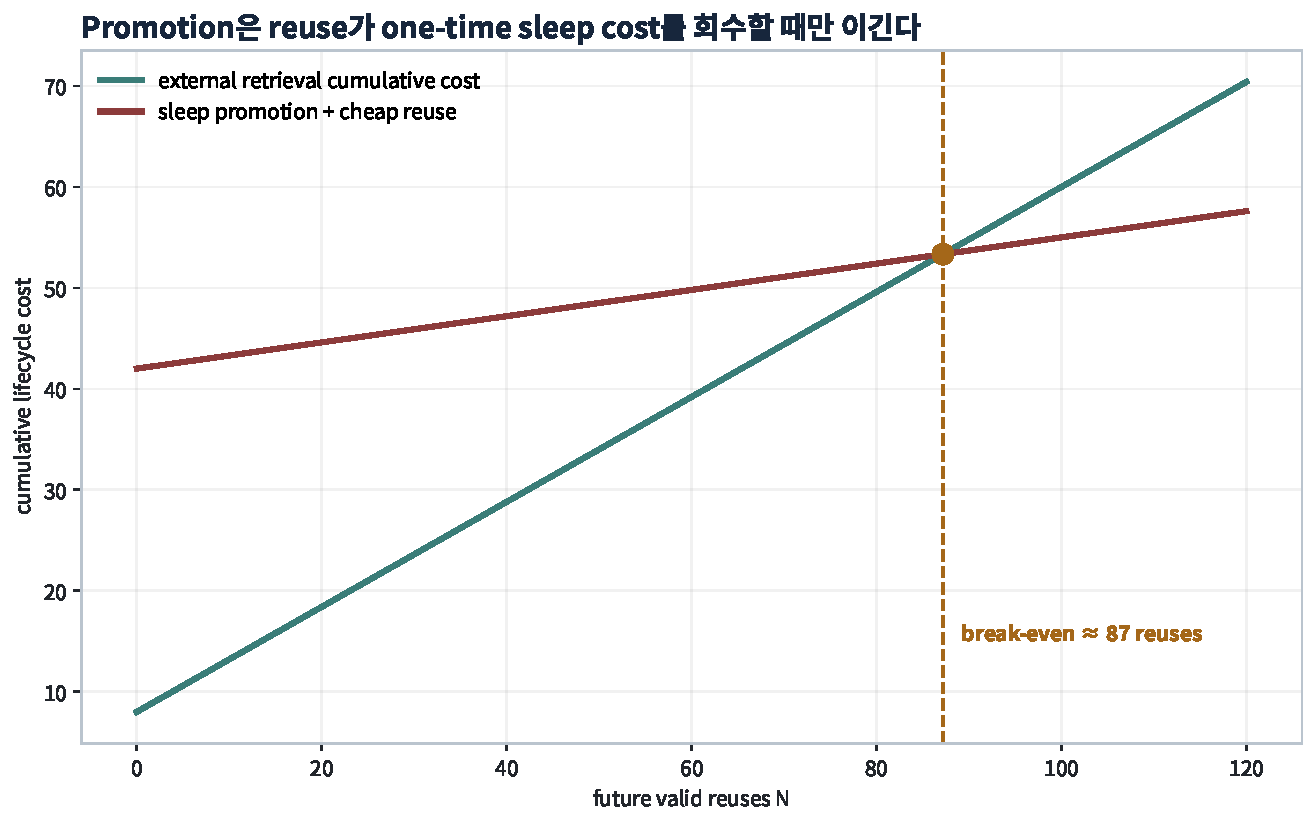
\includegraphics[width=0.96\textwidth]{figures/stc-f008.pdf}
  \caption{One-time sleep cost와 future valid reuse의 analytical crossover. Break-even 왼쪽은 external
  retrieval이, 오른쪽은 compiled artifact가 유리할 수 있다. Quality·governance 차이가 있으면 경계가
  이동한다.}
  \stcfigure{STC-F008}
  \figsource{Original analytical redraw; SRC-STC-0027, SRC-STC-0052}{초기 compile 비용을 수평선으로, reuse에 따라 누적되는 per-use saving을 상승선으로 나타낸 교차 그래프.}
  \label{fig:reuse-break-even}
\end{figure}

측정용 efficiency는 scalar를 강제하지 않고 먼저 Pareto vector로 보고한다.

\begin{align}
\eta_i={}&\frac{\Delta U_{later,i}\,R_{valid,i}}{C_{life,i}},\\
C_{life}={}&C_{ingest}+C_{transform}+C_{train}+C_{validate}\nonumber\\
&+C_{publish}+C_{serve}+C_{maint}+C_{delete/rollback}.
\end{align}

Dollar, joule, byte, second를 임의 환율로 합치지 않는다. Utility floor를 통과한 뒤 비용을 비교하거나,
cost cap 아래 utility를 비교하는 방식이 더 재현 가능하다.

\section{Finite state가 만드는 capacity knee}

고정된 finite state는 positive-entropy stream을 같은 distortion으로 영원히 보존할 수 없다. Mutable state가
$b_{mutable}$ bits이고 conditionally independent answer family의 rate--distortion cost가
$R_{Y_i\mid Q_i,\Theta_0}(D_i)$라면 제한된 조건 아래

\begin{equation}
\sum_{i=1}^{n}R_{Y_i\mid Q_i,\Theta_0}(D_i)
\le H(M_n\mid\Theta_0)\le b_{mutable}.
\end{equation}

이는 facts-per-parameter 보편 상수가 아니다. 하지만 계속 들어오는 novel evidence에 대해 state growth,
distortion 증가, forgetting, external offload 중 적어도 하나가 필요하다는 점은 분명히 한다.

Finite memory에서는 marginal consolidation utility가 떨어지고 interference, compaction 또는 delete cost가
급증하는 capacity knee가 나타날 것으로 예상된다.\claim{STC-C045}
\autocite{srcstc0034,srcstc0035,srcstc0036} Physical storage knee, normal-query reachability knee,
retrieval index knee, new-task plasticity knee, governance knee, hot-state residency knee는 서로 다른 위치에
있을 수 있다. 따라서 ``parameter가 아직 남았다''는 말은 behavioral capacity의 반증이 아니다.

\begin{figure}[htbp]
  \centering
  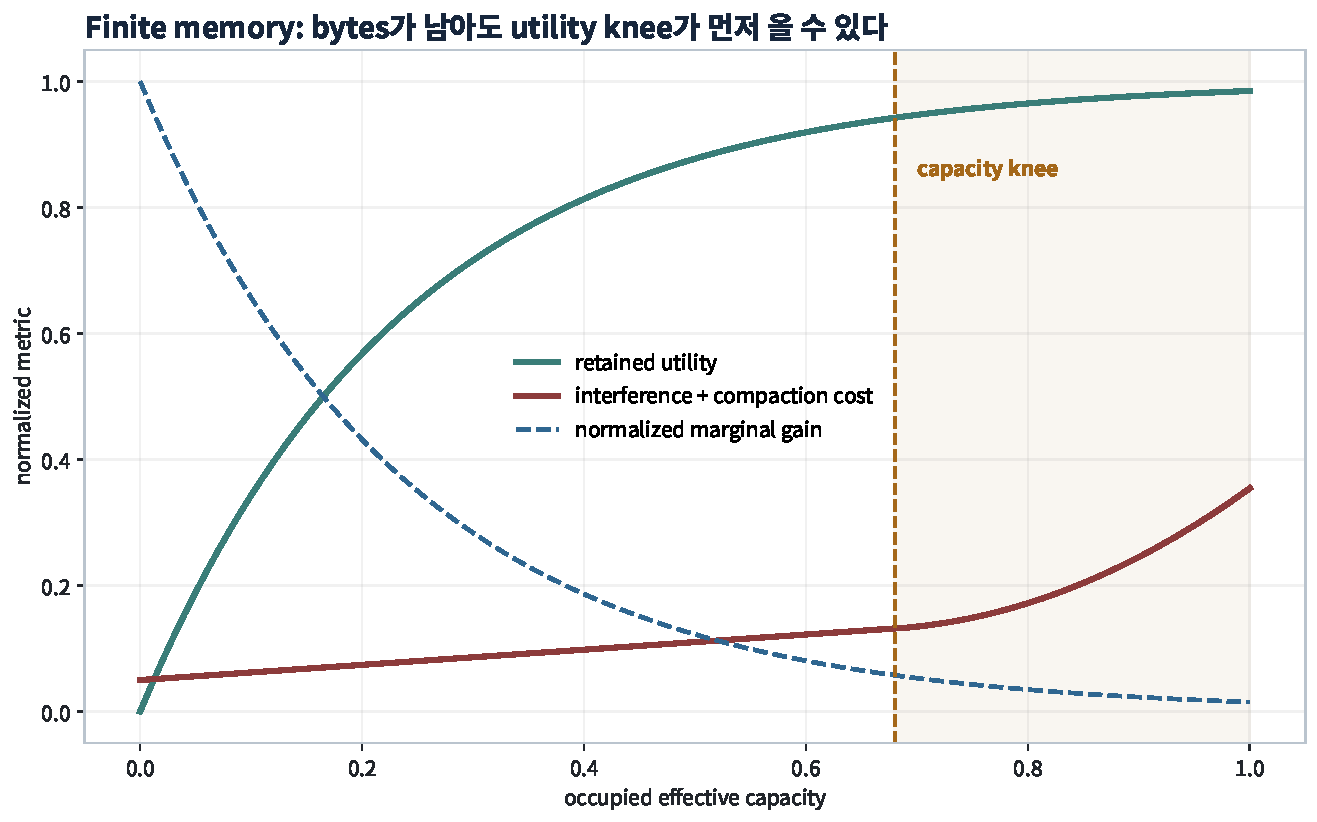
\includegraphics[width=0.96\textwidth]{figures/stc-f009.pdf}
  \caption{Finite-memory capacity knee의 가설적 형태. Physical occupancy가 한계에 닿기 전에 behavioral
  reachability 또는 plasticity가 임계값 아래로 내려갈 수 있다. 곡선은 설명용이며 측정 결과가 아니다.}
  \stcfigure{STC-F009}
  \figsource{Original hypothesis redraw; SRC-STC-0034, SRC-STC-0036}{Evidence load가 증가할 때 retention과 plasticity가 서로 다른 knee에서 감소하는 두 곡선.}
  \label{fig:capacity-knee}
\end{figure}

Controlled sweep에서는 retention threshold $\tau_{ret}$을 먼저 고정하고

\begin{equation}
\operatorname{logit}p_{ret}(N_a)=\operatorname{logit}\tau_{ret}
-\kappa\log(N_a/K_{eff})
\end{equation}

같은 segmented knee candidate와 generalized mean, min-bottleneck, monotone nonparametric competitor를
함께 맞춘다. 전 구간 power law 하나를 강제하지 않는다.

\section{Cadence와 queue의 내부 optimum}

Optimal cadence는 staleness, batching efficiency, interference와 wake-SLA impact를 균형시켜야 한다.
Continuous update나 무한히 긴 batch 어느 쪽도 일반적으로 최적이 아니다.\claim{STC-C044}
\autocite{srcstc0020,srcstc0022,srcstc0063}

Run cost $C_s$, interval $\tau$, smooth staleness penalty $a\tau^p$라는 제한에서

\begin{equation}
\bar C(\tau)=\frac{C_s}{\tau}+a\tau^p,
\qquad
\tau^*=\left(\frac{C_s}{ap}\right)^{1/(p+1)}.
\label{eq:cadence-optimum}
\end{equation}

Event rate $r_e$, fixed job cost $F$, linear delay harm $h$이면
$\tau^*=\sqrt{2F/(hr_e)}$다. Burst arrival, hard deadline, multi-resource blocking, capacity-triggered
regime change에서는 이 closed form이 깨진다. 이때 queue recursion
$Q_{t+1}=\max\{0,Q_t+A_t-S_t\}$와 P99 job age를 직접 시뮬레이션해야 한다.

\begin{figure}[htbp]
  \centering
  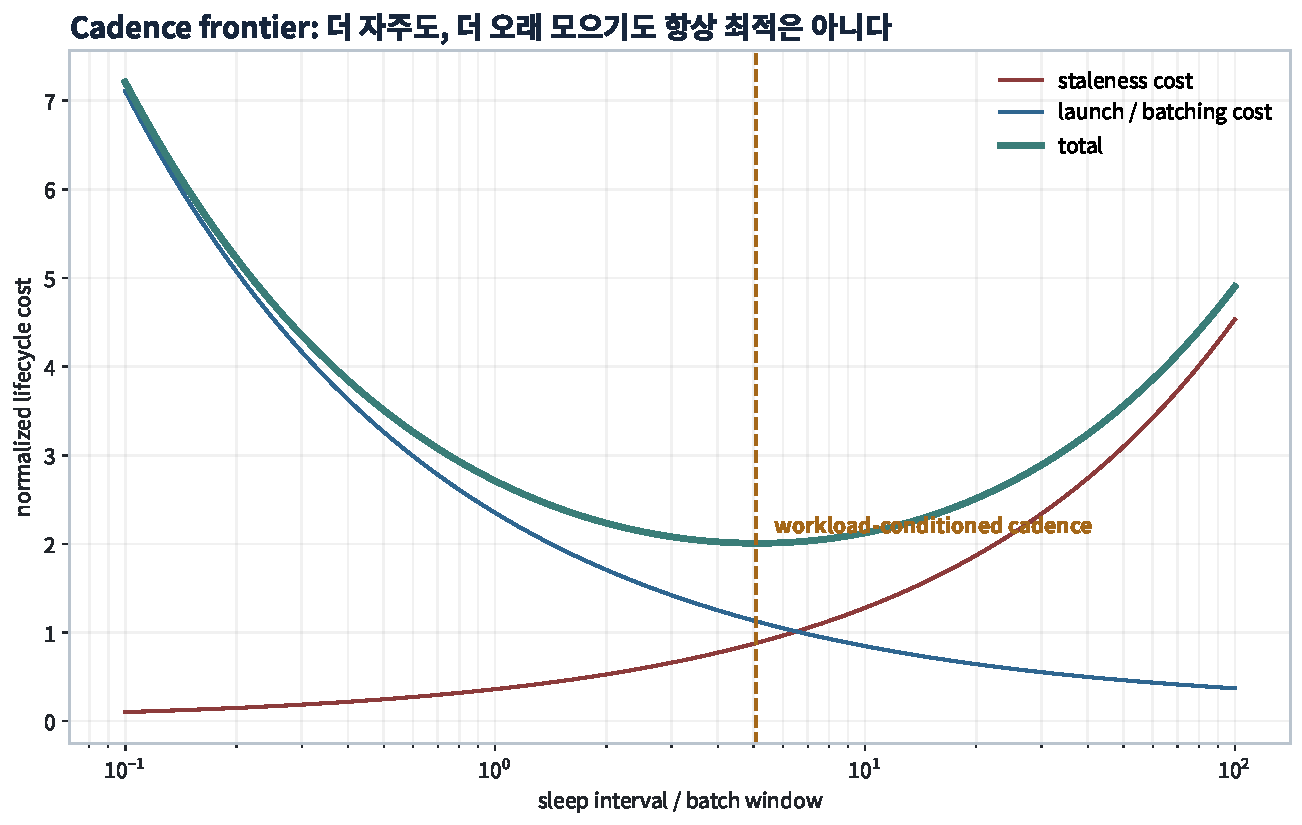
\includegraphics[width=0.96\textwidth]{figures/stc-f010.pdf}
  \caption{Cadence frontier. 너무 잦은 sleep은 fixed overhead와 interference가 크고, 너무 늦은 sleep은
  staleness와 queue age가 크다. 내부 optimum의 위치는 workload와 resource vector에 따라 변한다.}
  \stcfigure{STC-F010}
  \figsource{Original analytical redraw; SRC-STC-0020, SRC-STC-0063}{짧은 interval의 batching 비용과 긴 interval의 staleness 비용이 합쳐져 U자 total cost를 만드는 그래프.}
  \label{fig:cadence-frontier}
\end{figure}

\section{Fit candidate와 법칙 승격 조건}

첫 fit candidate는 saturating return에 interference, staleness, risk penalty를 분리한다.

\begin{equation}
\Delta U=A\left[1-\exp\left(-kF_s^{\alpha}E_{eff}^{\beta}R_v^{\gamma}\right)\right]
-\Phi_{int}-\Phi_{stale}-\Phi_{risk}.
\end{equation}

$E_{eff}$는 authorization, confidence, diversity를 통과한 canonical evidence이고 $R_v$는 valid future
reuse다. Competitor는 log-linear, floor가 있는 power law, segmented knee, generalized mean,
nonparametric monotone surface다. Sign change나 knee가 보이면 global power law를 기각한다.

진짜 STC scaling law라 부르려면 (1) unit과 state boundary를 고정하고, (2) model size·workload·medium·
hardware를 둘 이상 포함하며, (3) strongest alternative와 total lifecycle cost를 맞추고, (4) held-out
condition을 예측하고, (5) knee를 숨기지 않으며, (6) contamination·recursive depth·capacity·cycle control을
통과하고, (7) 실패한 형태를 공개해야 한다. 그 전까지의 정직한 산출물은 identity, restricted
break-even, workload-conditioned empirical surface와 falsifiable hypothesis다.
